\documentclass[11pt]{article}

\usepackage[letterpaper,margin=0.75in]{geometry}
\usepackage{booktabs}
\usepackage{caption}
\usepackage{graphicx}
\usepackage{listings}
\usepackage{float}
\usepackage{scrextend}
\usepackage{hyperref}
\usepackage[parfill]{parskip}
\renewcommand{\lstlistingname}{Snippet}


\begin{document}

\lstset{
  language=Python,
  basicstyle=\small,          % print whole listing small
  keywordstyle=\bfseries,
  identifierstyle=,           % nothing happens
  commentstyle=,              % white comments
  stringstyle=\ttfamily,      % typewriter type for strings
  showstringspaces=false,     % no special string spaces
  numbers=left,
  numberstyle=\tiny,
  numbersep=5pt,
  frame=tb
}

\title{Congestion Control Part 2}

\author{Brandt Elison & Joe Eklund}

\date{March 31, 2016}

\maketitle

\section{Introduction}

The purpose of our project was to verify our implementation of TCP congestion control by testing using a series of experiments. We divided our experiments into two categories: basic and advanced. The basic experiments tested the performance of our implementation of TCP congestion control by varying the number of flows that concurrently transfer a 1 MB file over a single link between two hosts. The advanced experiments also manipulated the link congestion, but they altered the network topology and the way TCP responded to loss events.

\section{Basic Experiments}

For our basic experiments we created a two host network with the following parameters:

\begin{itemize}
  \item 10 ms - propagation delay
  \item 100 packets - queue size
  \item 10 Mbps - transmission rate
  \item 500,000 bytes - intitial slow start threshold
\end{itemize}

Each of the experiments uses a different number of flows, meaning a different number of connections transfering 1 MB files simultaneously on the link.

\subsection{One Flow}
  
\begin{figure}[H]
\caption{The graph of our one flow receiver's rate over time.}
	\label{figure1}
  	\centering
  	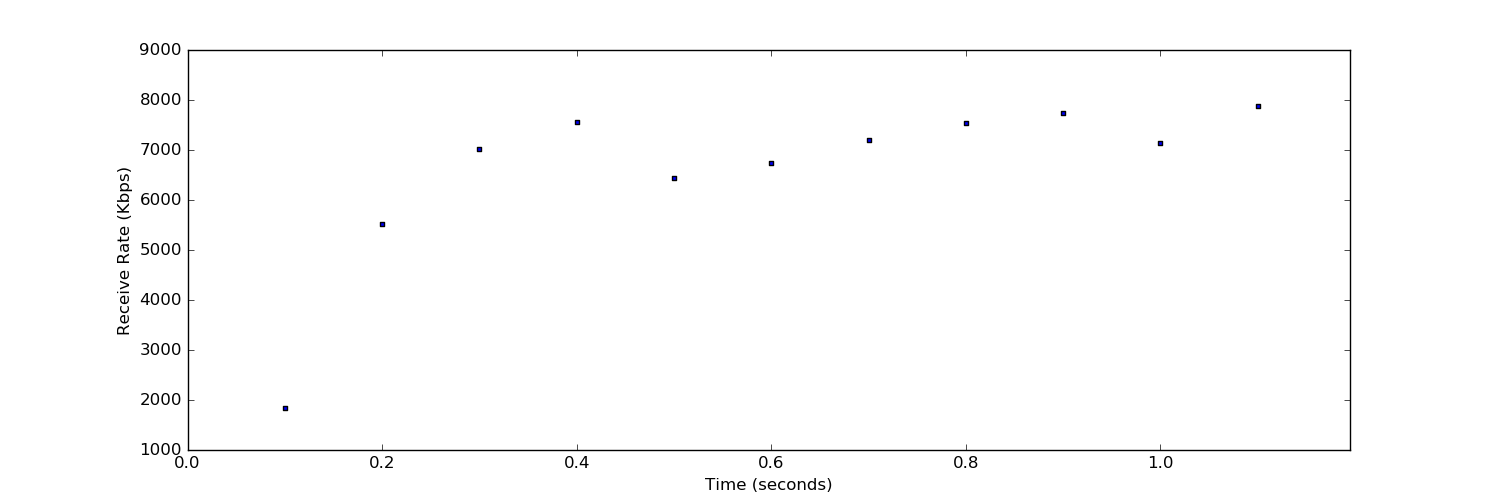
\includegraphics[width=\linewidth]{1f_rate.png}
\end{figure}

\begin{figure}[H]
\caption{The graph of our one flow queue size over time.}
  \label{figure2}
    \centering
    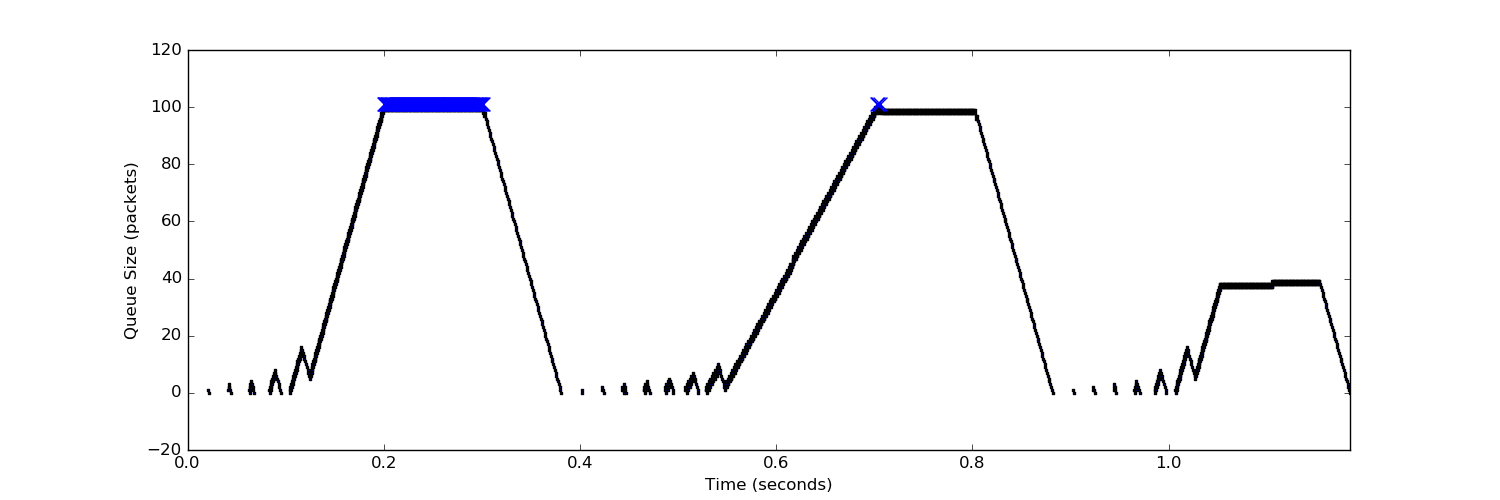
\includegraphics[width=\linewidth]{1f_queue.png}
\end{figure}

\begin{figure}[H]
\caption{The graph of our one flow congestion window size over time.}
  \label{figure3}
    \centering
    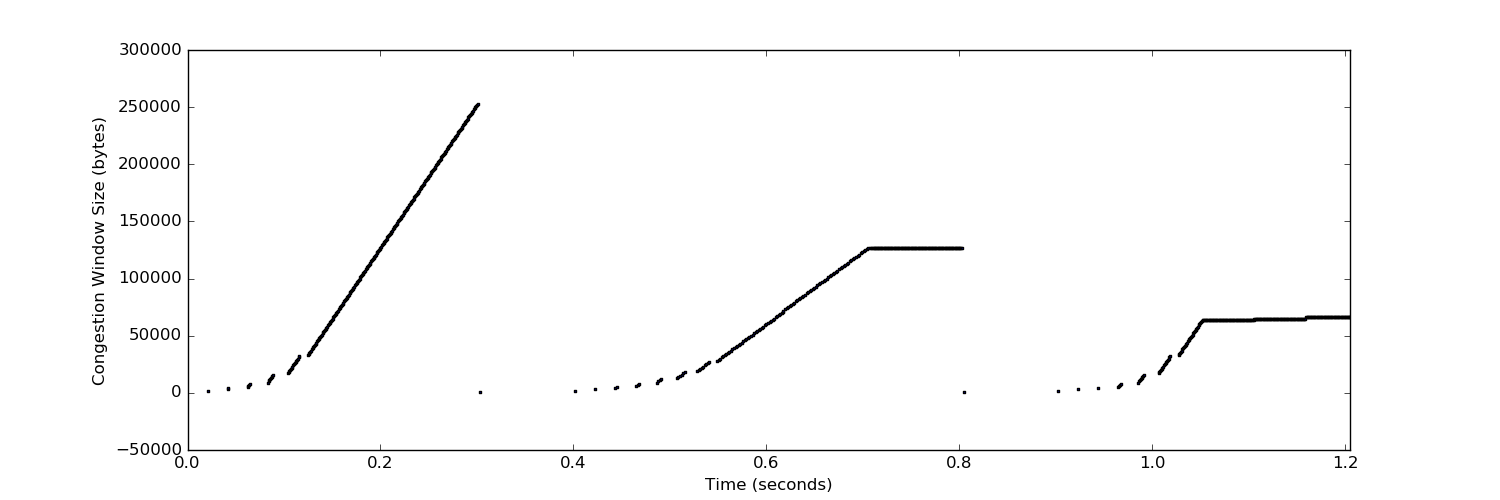
\includegraphics[width=\linewidth]{1f_window.png}
\end{figure}

\begin{figure}[H]
\caption{The graph of our one flow sequence plot.}
  \label{figure4}
    \centering
    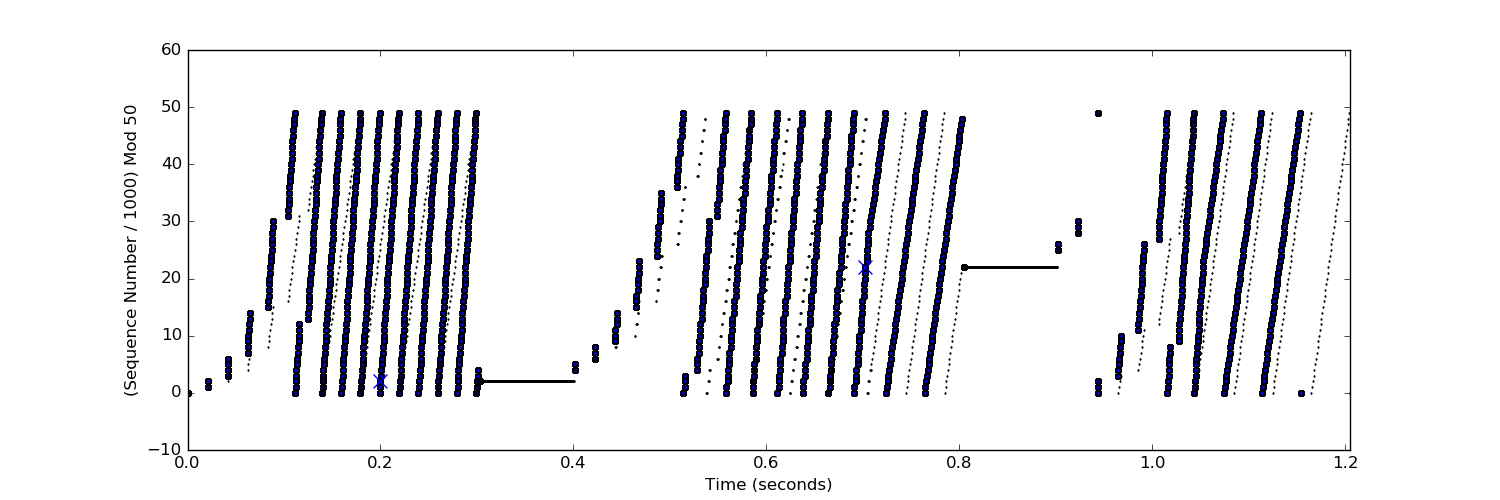
\includegraphics[width=\linewidth]{1f_seq.png}
\end{figure}

Figure 1 shows how the receive rate changes over time for a single flow. We can see that the receive rate goes up very quickly and levels off; this is expected behavior because the flow has access to the full bandwidth. In Figure 2 we see how the queue size is quickly filled during slow start because the threshold is much larger than the queue size. However after some loss, congestion control helps keep the queue size under its max of 100 packets. If the file that we transfered was larger than 1 MB, we would see the additive increase section at around 1.1 seconds continue without loss for a long time. Figure 3 supports Figure 2 by showing the typical saw tooth pattern that reflects TCP's attempt to find a congestion window size appropriate for the link. 

\subsection{Two Flow}

\begin{figure}[H]
\caption{The graph of our two flow receivers' rates over time.}
  \label{figure5}
    \centering
    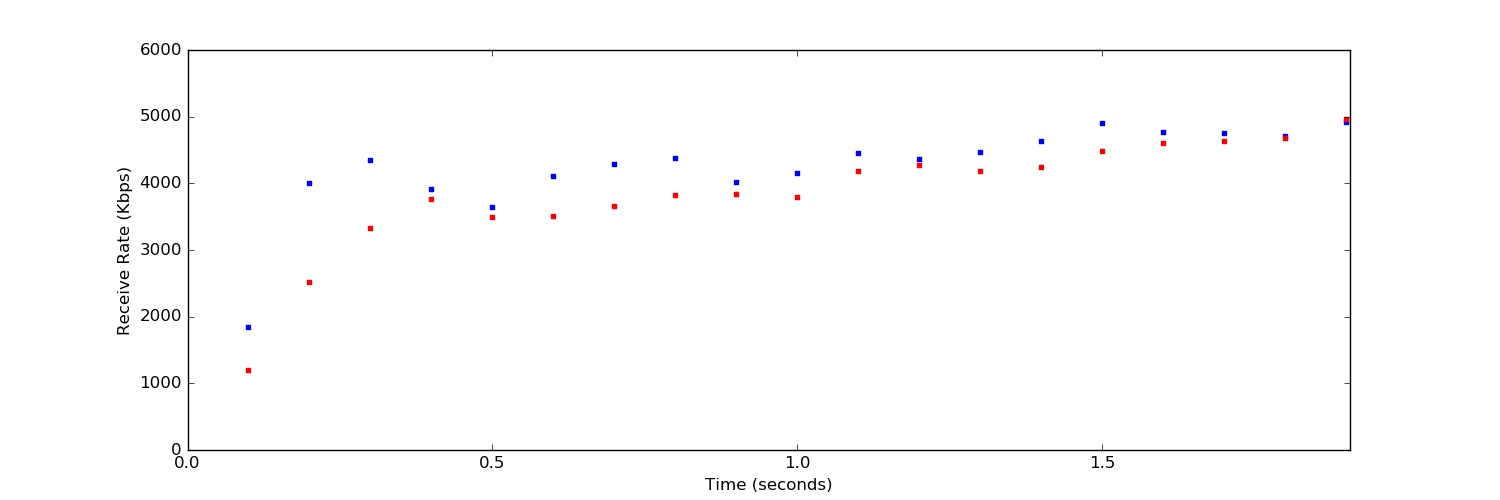
\includegraphics[width=\linewidth]{2f_rate.png}
\end{figure}

\begin{figure}[H]
\caption{The graph of our two flow queue size over time.}
  \label{figure6}
    \centering
    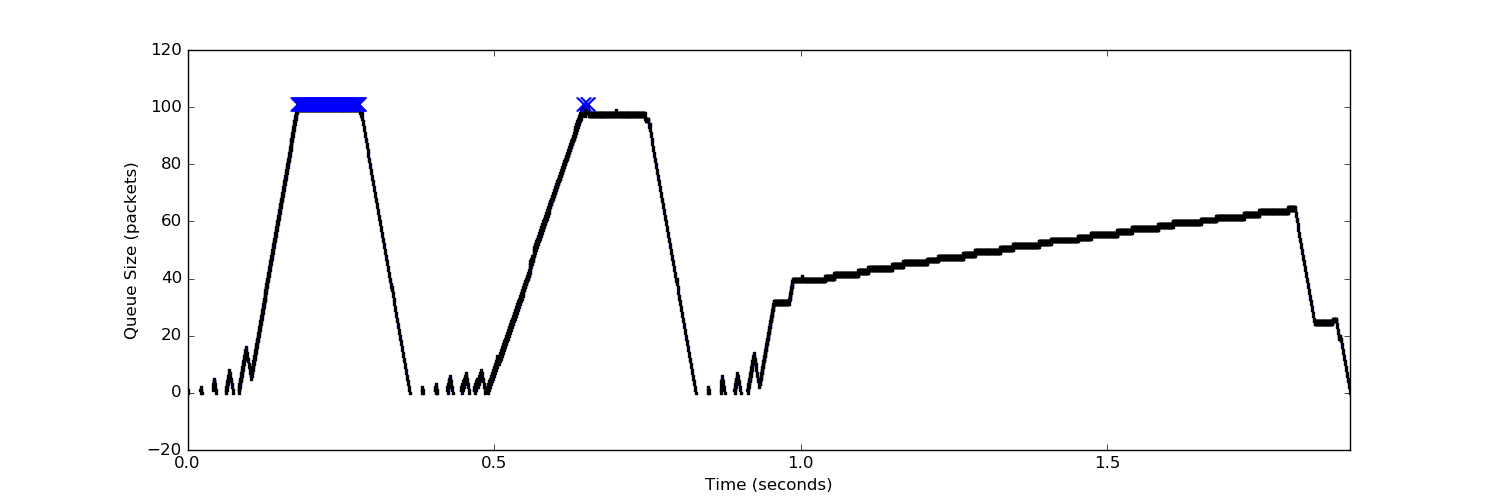
\includegraphics[width=\linewidth]{2f_queue.png}
\end{figure}

\begin{figure}[H]
\caption{The graph of our two flow congestion window size over time for flow A.}
  \label{figure7}
    \centering
    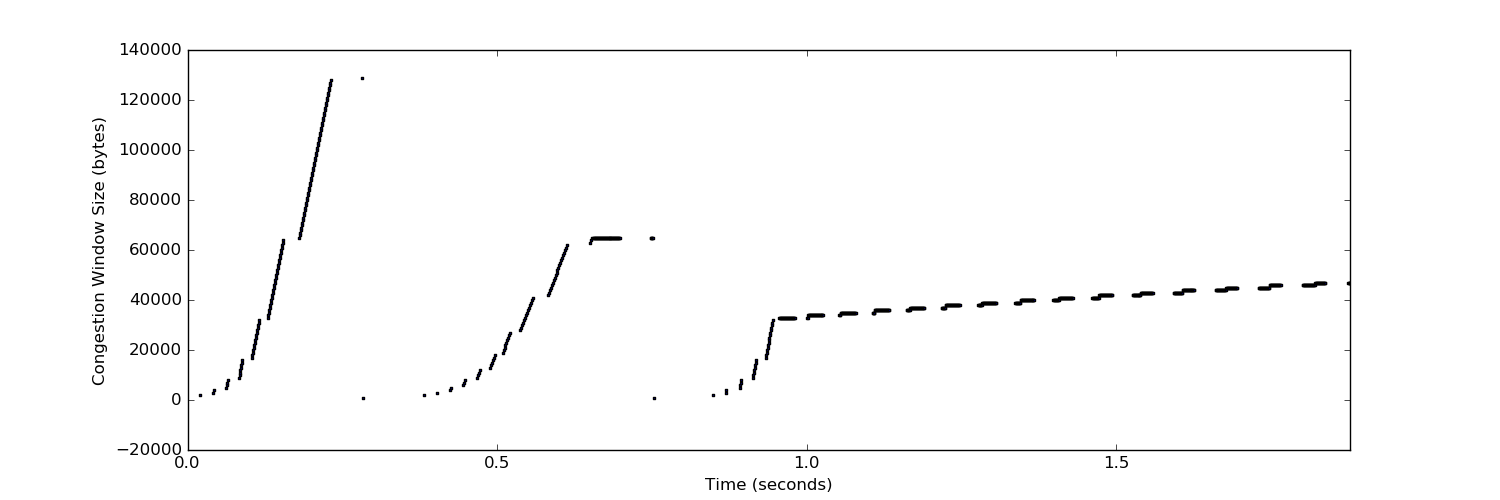
\includegraphics[width=\linewidth]{2f1_window.png}
\end{figure}

\begin{figure}[H]
\caption{The graph of our two flow congestion window size over time for flow B.}
  \label{figure8}
    \centering
    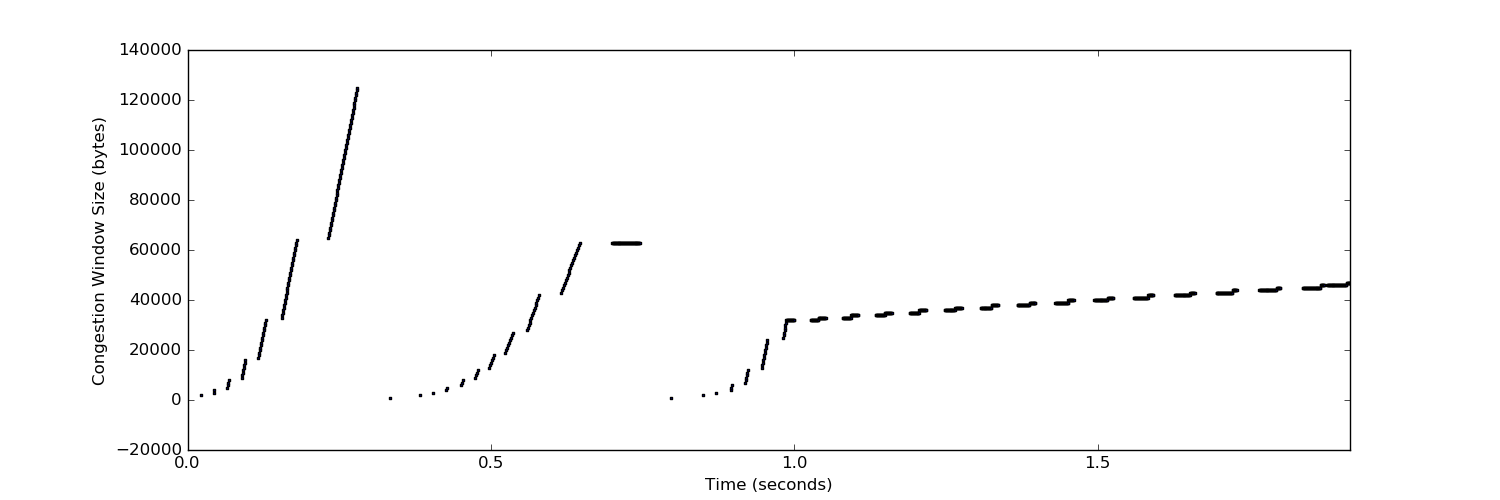
\includegraphics[width=\linewidth]{2f2_window.png}
\end{figure}

\begin{figure}[H]
\caption{The graph of our two flow sequence plot for flow A.}
  \label{figure9}
    \centering
    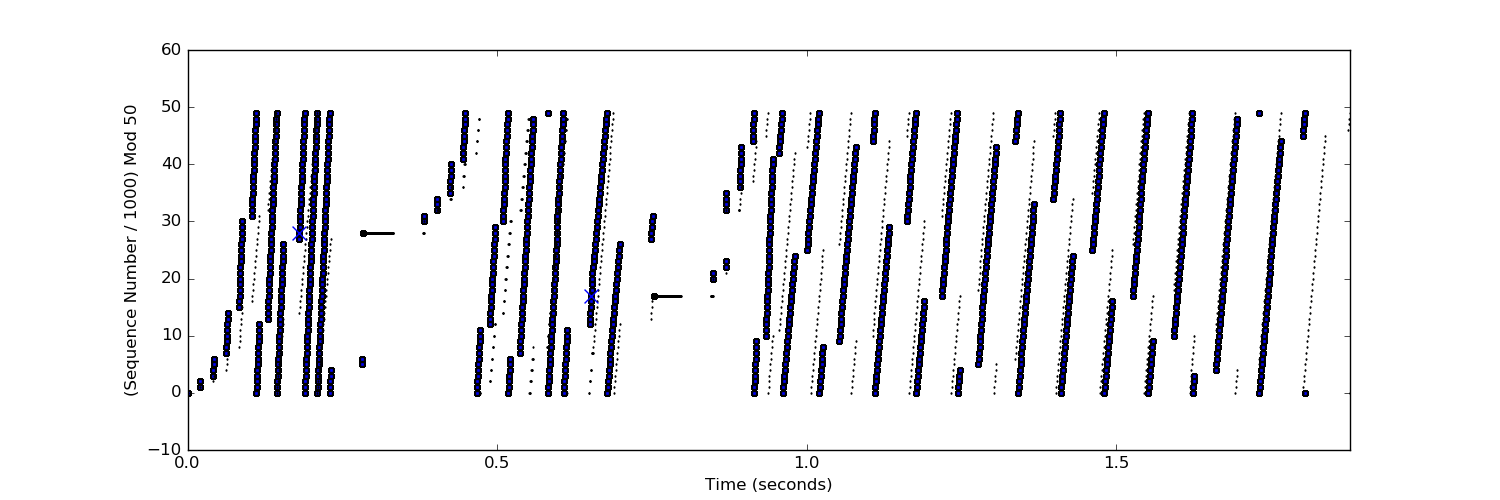
\includegraphics[width=\linewidth]{2f1_seq.png}
\end{figure}

\begin{figure}[H]
\caption{The graph of our two flow sequence plot for flow B.}
  \label{figure10}
    \centering
    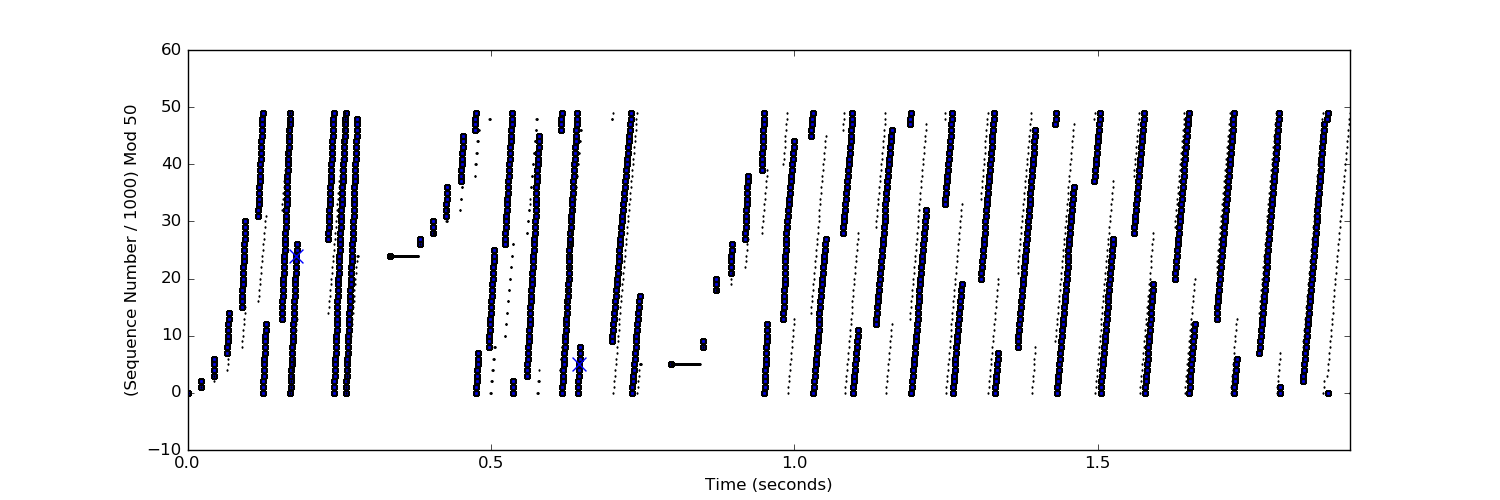
\includegraphics[width=\linewidth]{2f2_seq.png}
\end{figure}

Because the two flows in this experiment were identical, we would expect both data series in Figure 5 to look nearly identical. Figure 5 shows this behavior. We would also expect Figures 7 and 8 to look nearly identical because both flows experience loss at nearly the same time and adjust their windows to the same values. Figures 7 and 8 do look nearly identical as expected. Figure 6 also demonstrates expected behavior; this is clear particularly when you compare Figure 6 with Figure 2. On both graphs we see two peaks loss events occuring while TCP is still identifying a good window for the link. After the second peak both flows start additive increase before the queue is filled. However, in Figure 6 the slope of the increase in queue size during the additive increase period is steeper than the slope in Figure 2 because Figure 6 shows two flows, both doing additive increase. 

\subsection{Five Flow}

\begin{figure}[H]
\caption{The graph of our five flow receivers' rates over time.}
  \label{figure11}
    \centering
    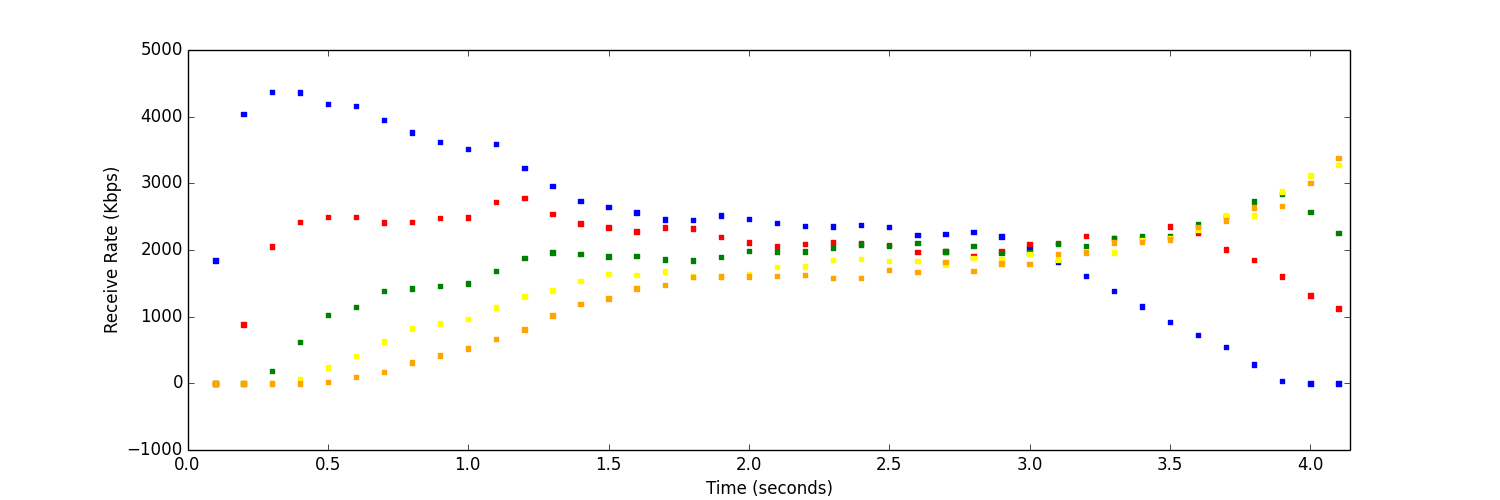
\includegraphics[width=\linewidth]{5f_rate.png}
\end{figure}

\begin{figure}[H]
\caption{The graph of our five flow queue size over time.}
  \label{figure12}
    \centering
    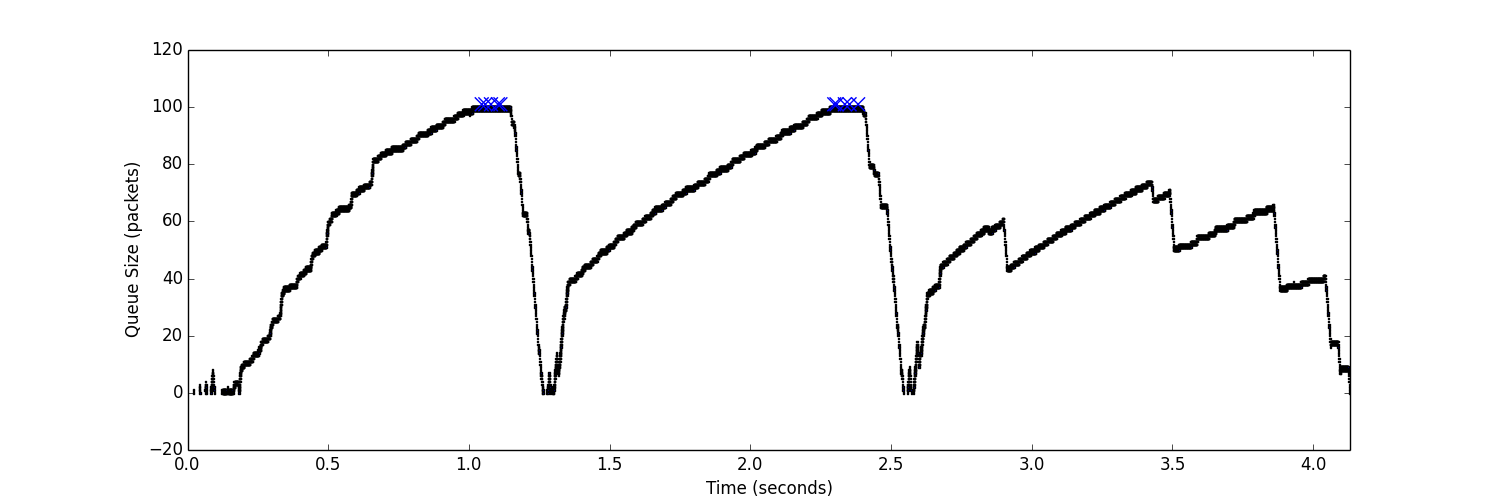
\includegraphics[width=\linewidth]{5f_queue.png}
\end{figure}

For five flow we decided a smaller threshold size of 16,000 bytes. We chose to do this because with such a small file there was not enough time for the TCP connections to balance their share of the link before flows started finishing their file transfer. Five flow also differed from one and two flow because each flow began transfering 0.1 seconds after the preceeding flow (i.e. 0.0, 0.1, 0.2, 0.3, 0.4).

In a correct implementation of TCP, the first flow to begin transferring will immedietely take advantage of all the bandwidth. As more connections begin sharing the link the receive rate of the initial flows should drop while the receive rate of the newer flows should increase until they are roughly the same. This means that they are equally sharing the bandwidth. As early flows finish transferring their files the remaining flows start to take advantage of the newly available bandwidth. Figure 11 is evidence of this behavior. 

\section{Advanced Experiments}


\subsection{Additive Increase - Additive Decrease (AIAD)}

\begin{figure}[H]
\caption{The graph of our one flow receiver's rate over time with AIAD.}
  \label{figure13}
    \centering
    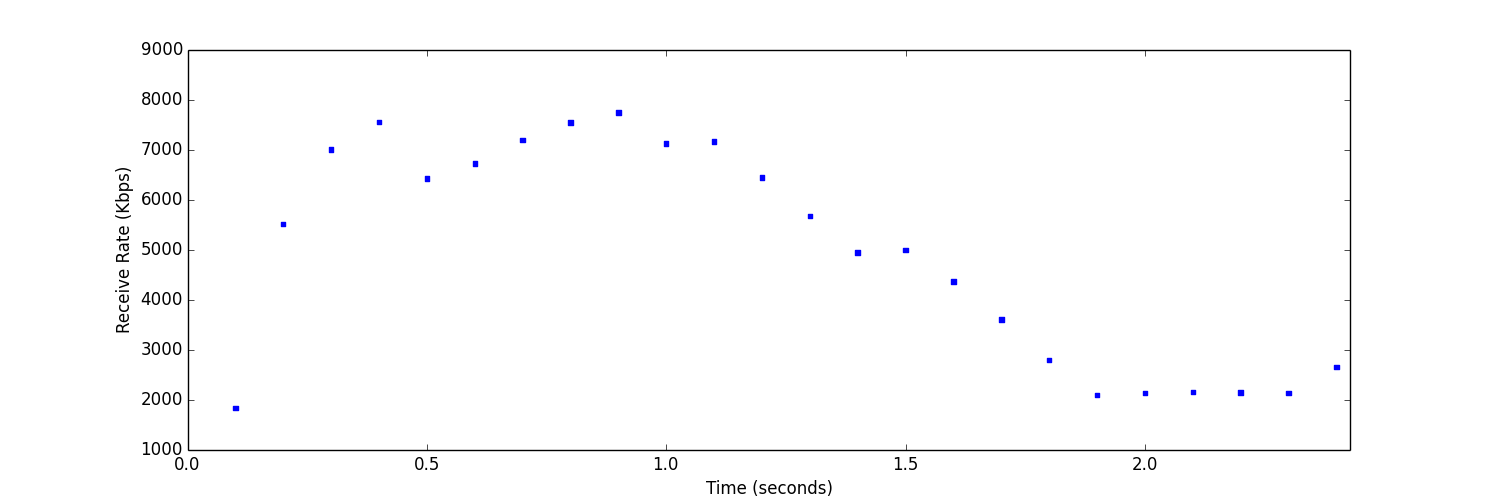
\includegraphics[width=\linewidth]{1f_rateAIAD.png}
\end{figure}

\begin{figure}[H]
\caption{The graph of our one flow congestion window size over time with AIAD.}
  \label{figure14}
    \centering
    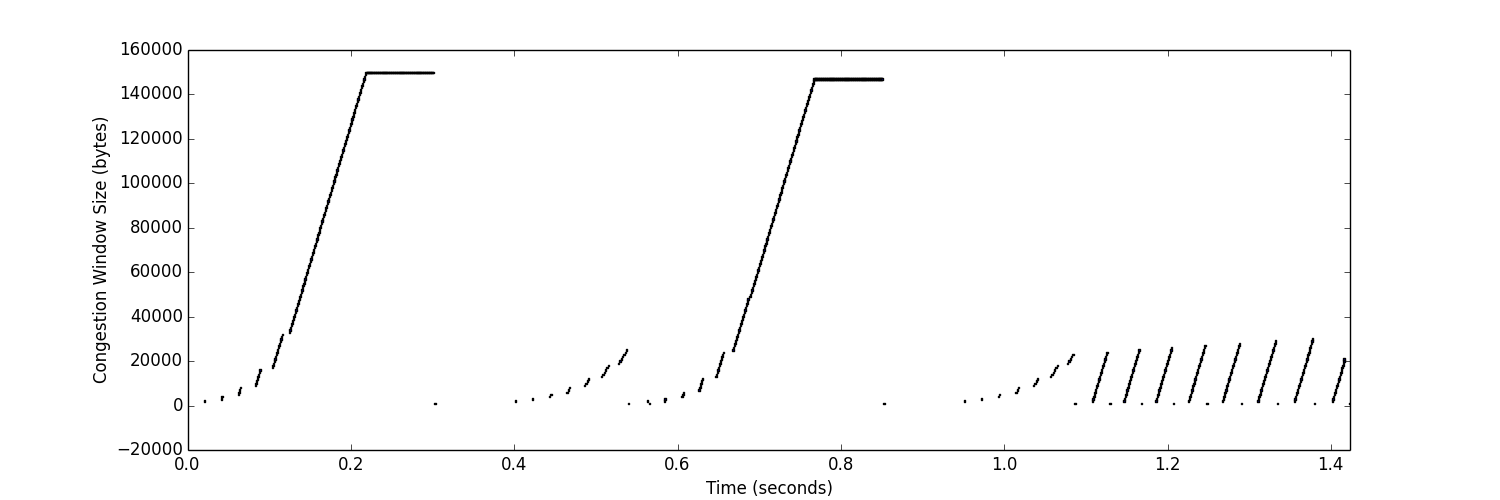
\includegraphics[width=\linewidth]{1f_windowAIAD.png}
\end{figure}


discuss AIAD here

\subsection{Additve Increase - 5/6 Multiplicative Decrease (AIMD)}

\begin{figure}[H]
\caption{The graph of our one flow receiver's rate over time with a 5/6 multiplicative decrease.}
  \label{figure15}
    \centering
    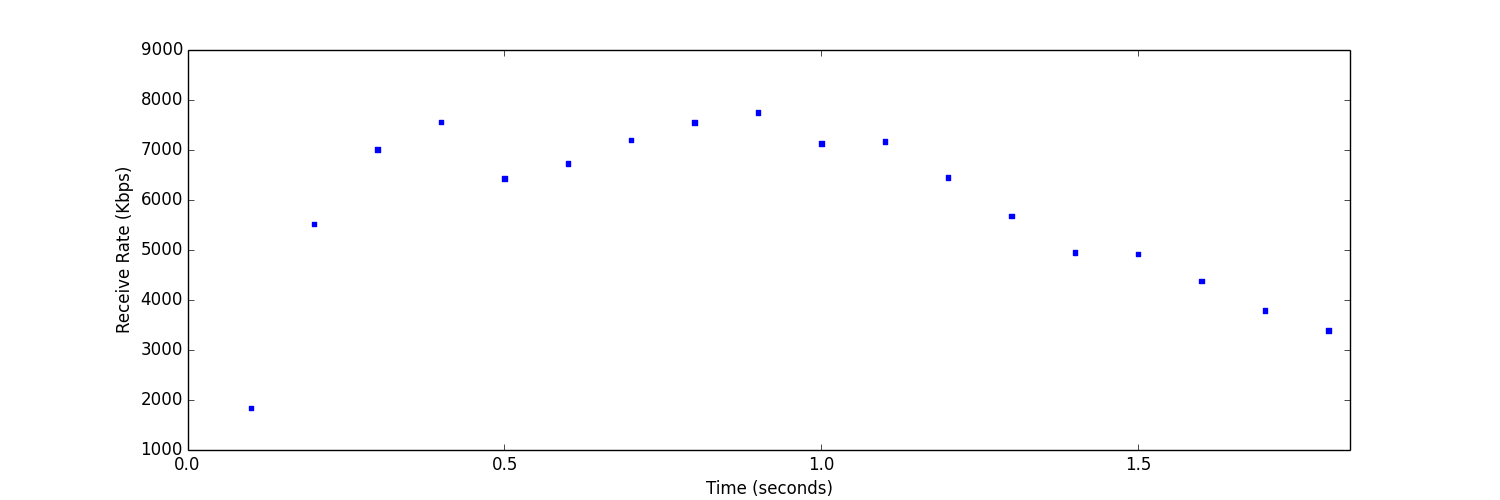
\includegraphics[width=\linewidth]{1f_rateAIMD.png}
\end{figure}

\begin{figure}[H]
\caption{The graph of our one flow congestion window size over time with a 5/6 multiplicative decrease.}
  \label{figure16}
    \centering
    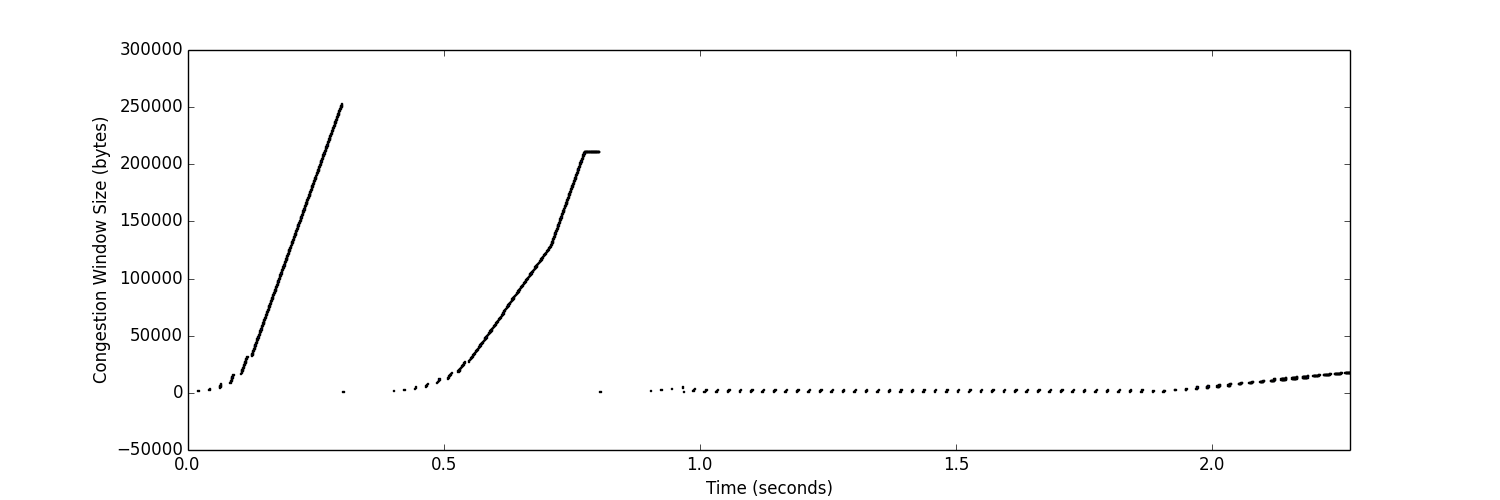
\includegraphics[width=\linewidth]{1f_windowAIMD.png}
\end{figure}

discuss AIMD here

\subsection{Competing AIMD}

\begin{figure}[H]
\caption{The graph of our two flow receivers' rates over time with competing AIMD.}
  \label{figure15}
    \centering
    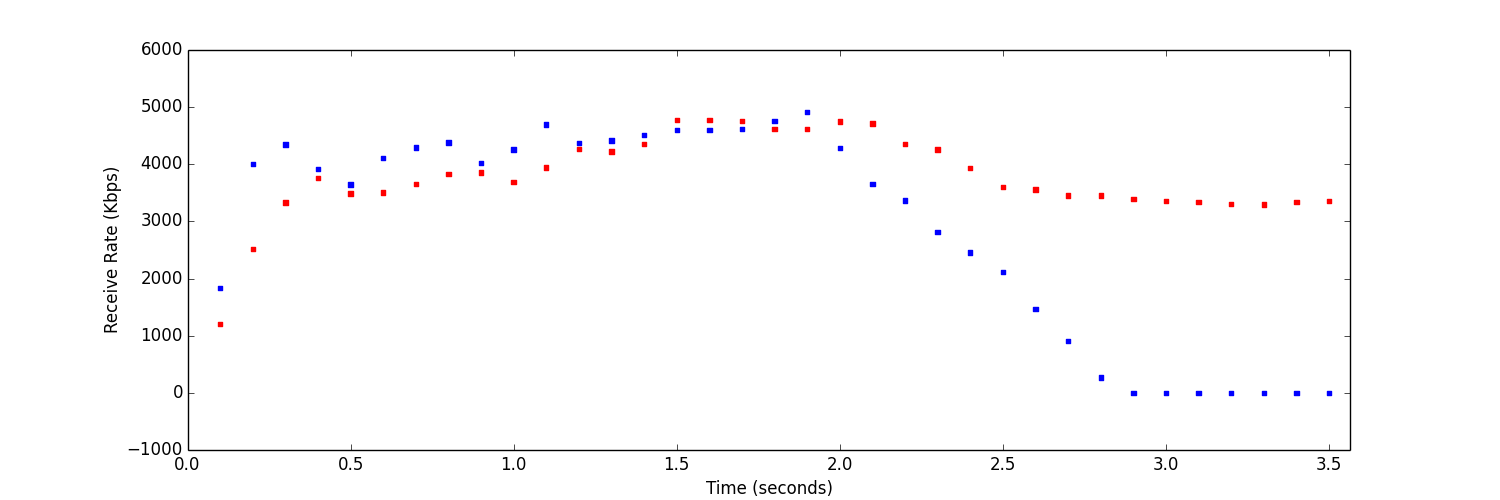
\includegraphics[width=\linewidth]{2f_rateAIMD.png}
\end{figure}

discuss competing AIMD here

\subsection{Competing Round Trip Time (RTT)}

\begin{figure}[H]
\caption{The graph of our two flow receivers' rates over time with competing RTT.}
  \label{figure16}
    \centering
    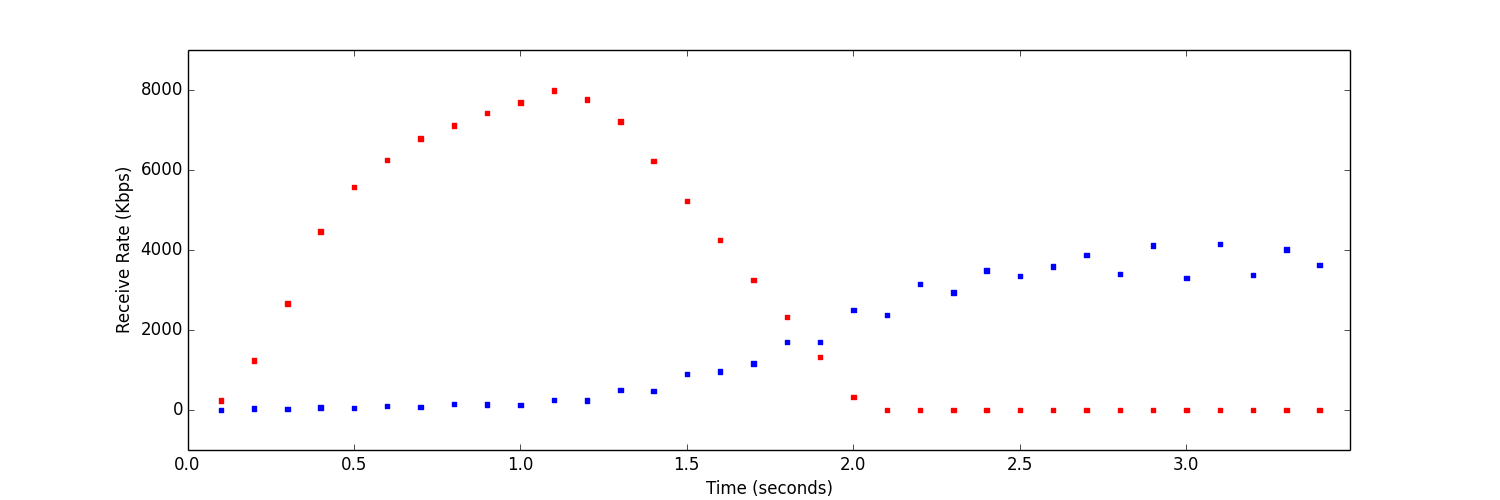
\includegraphics[width=\linewidth]{2f_rate_rtt.png}
\end{figure}

discuss competing RTT here


\end{document}
